\documentclass{article}
\usepackage{../../Self_Style}

\title{Phys 20AL Week 6: Driven Harmonic Oscillator}
\author{Zih-Yu Hsieh}
\date{\today}

\begin{document}
\maketitle

\section{Aim of Experiment}
The experiment is aiming to observe how the natural frequency of a harmonic oscillator would affect its amplitude and phase differrence, when providing a driven force to the harmonic oscillators.

\hfil

\section{Experimental Setup (insert image)}
The equipments included: A large stand (with multiple clamps provided), a heavy mass of $0.5$ kg (used as driven source of the harmonic oscillator), metal wire, multiple strings (total of 12), multiple light masses (total of 11, used as pendulums), scissors, tapes, two meter sticks, and phones.

The setup will follow the steps below:
\begin{itemize}
    \item[1.] Tie the metal wire horizontally on the stand, and ensure it's tight enough.
    \item[2.] Use one of the strings to tie the heavy mass (0.5 kg) onto the metal wire (near one end of the wire), and tape it to ensure the metal wire would obtain some rotational motion when the heavy mass is swinging.
    \item[3.] Tie the light masses onto the wire. Ensure that they're spaced (so the pendulum motion would affect each other), while also close enough to the heavy mass (so the driven force caused by the heavy mass wouldn't be dissipated). Also, keep in mind of making each light mass pendulum with a different length, and with at least one having the same length as the heavy mass.
    \item[4.] Setup the two meter sticks below the pendulums: Fix one directly under the heavy mass, and fix the other meter stick directly under the light mass that's the farthest away from the heavy mass.
    \item[6.] Fix the phone at the other end of the stand, making sure the camera captures all pendulums, having all the masses are aligned in the center, and also including the meter sticks in the view of the camera. 
\end{itemize}

\begin{figure}[h!]
    \centering
    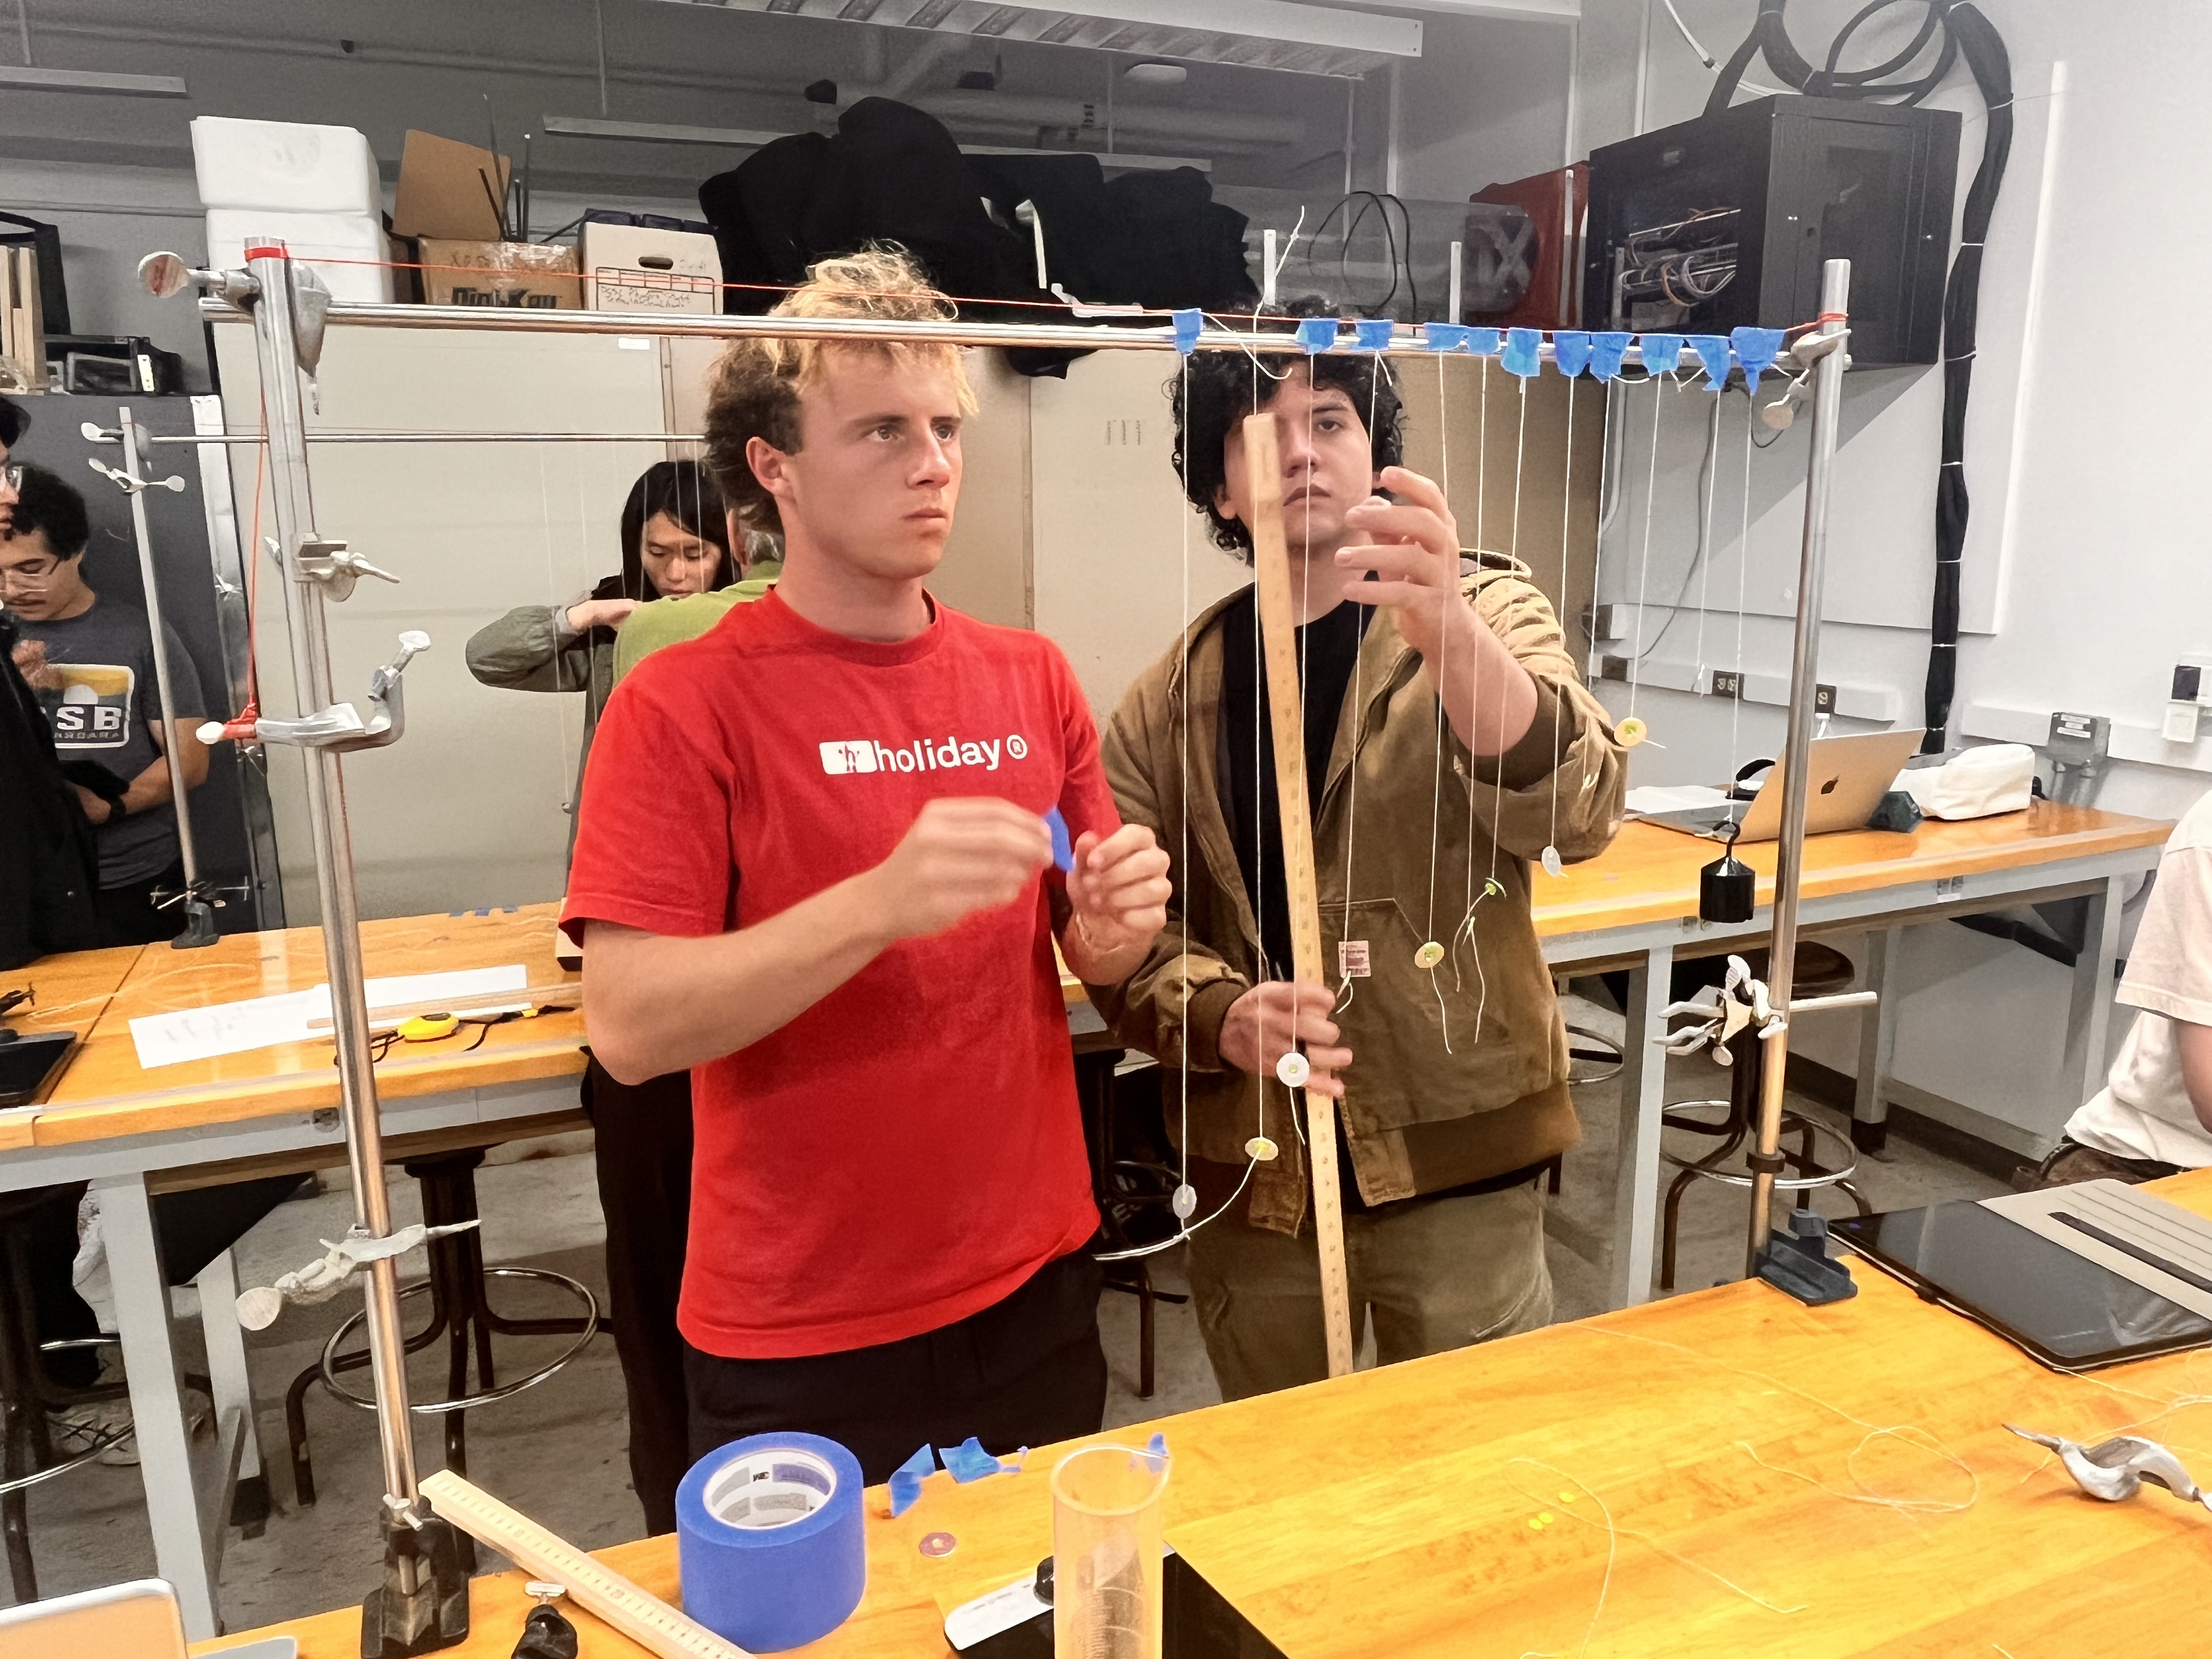
\includegraphics[width=100mm]{lab_setup_6.png}
\end{figure}

\newpage

\section{Quantity to Measure \& Method of Measurement}
In this experiment, we'll record a total of three trials. It is aimed to measure two quantities: The amplitudes of all the pendulum, and the phase difference.

For both amplitudes and phase difference, we'll record the whole process at stable state using camera. Then, the meter stick will serve as a metric to measure the amplitude of each pendulum; also, the time stamp of the video recording will serve as a source for measuring the time difference between the moment when each pendulum reaches maximum amplitude (vs. the moment when the driven pendulum reaches its maximum).

\hfil

\section{Experimental Procedure}
We'll follow hte procedure below:
\begin{itemize}
    \item[1.] Put the whole system at static equilibrium (having none of the pendulums actually moving), and raise the heavy mass to about $10$ cm away from equilibrium.
    \item[2.] Release the heavy mass pendulum, and wait until the system to reach a stable state.
    \item[3.] When the system reaches stable state, start recording, and let all the pendulums finish at least 5 to 6 cyclees.  
    \item[4.] Repeat Step 1 to 3 for a total of three trials. 
\end{itemize}

\hfil

\section{Experimental Data}
Here are the collected data (having amplitudes first in green, then having phase difference in purple):
\begin{figure}[h!]
    \centering
    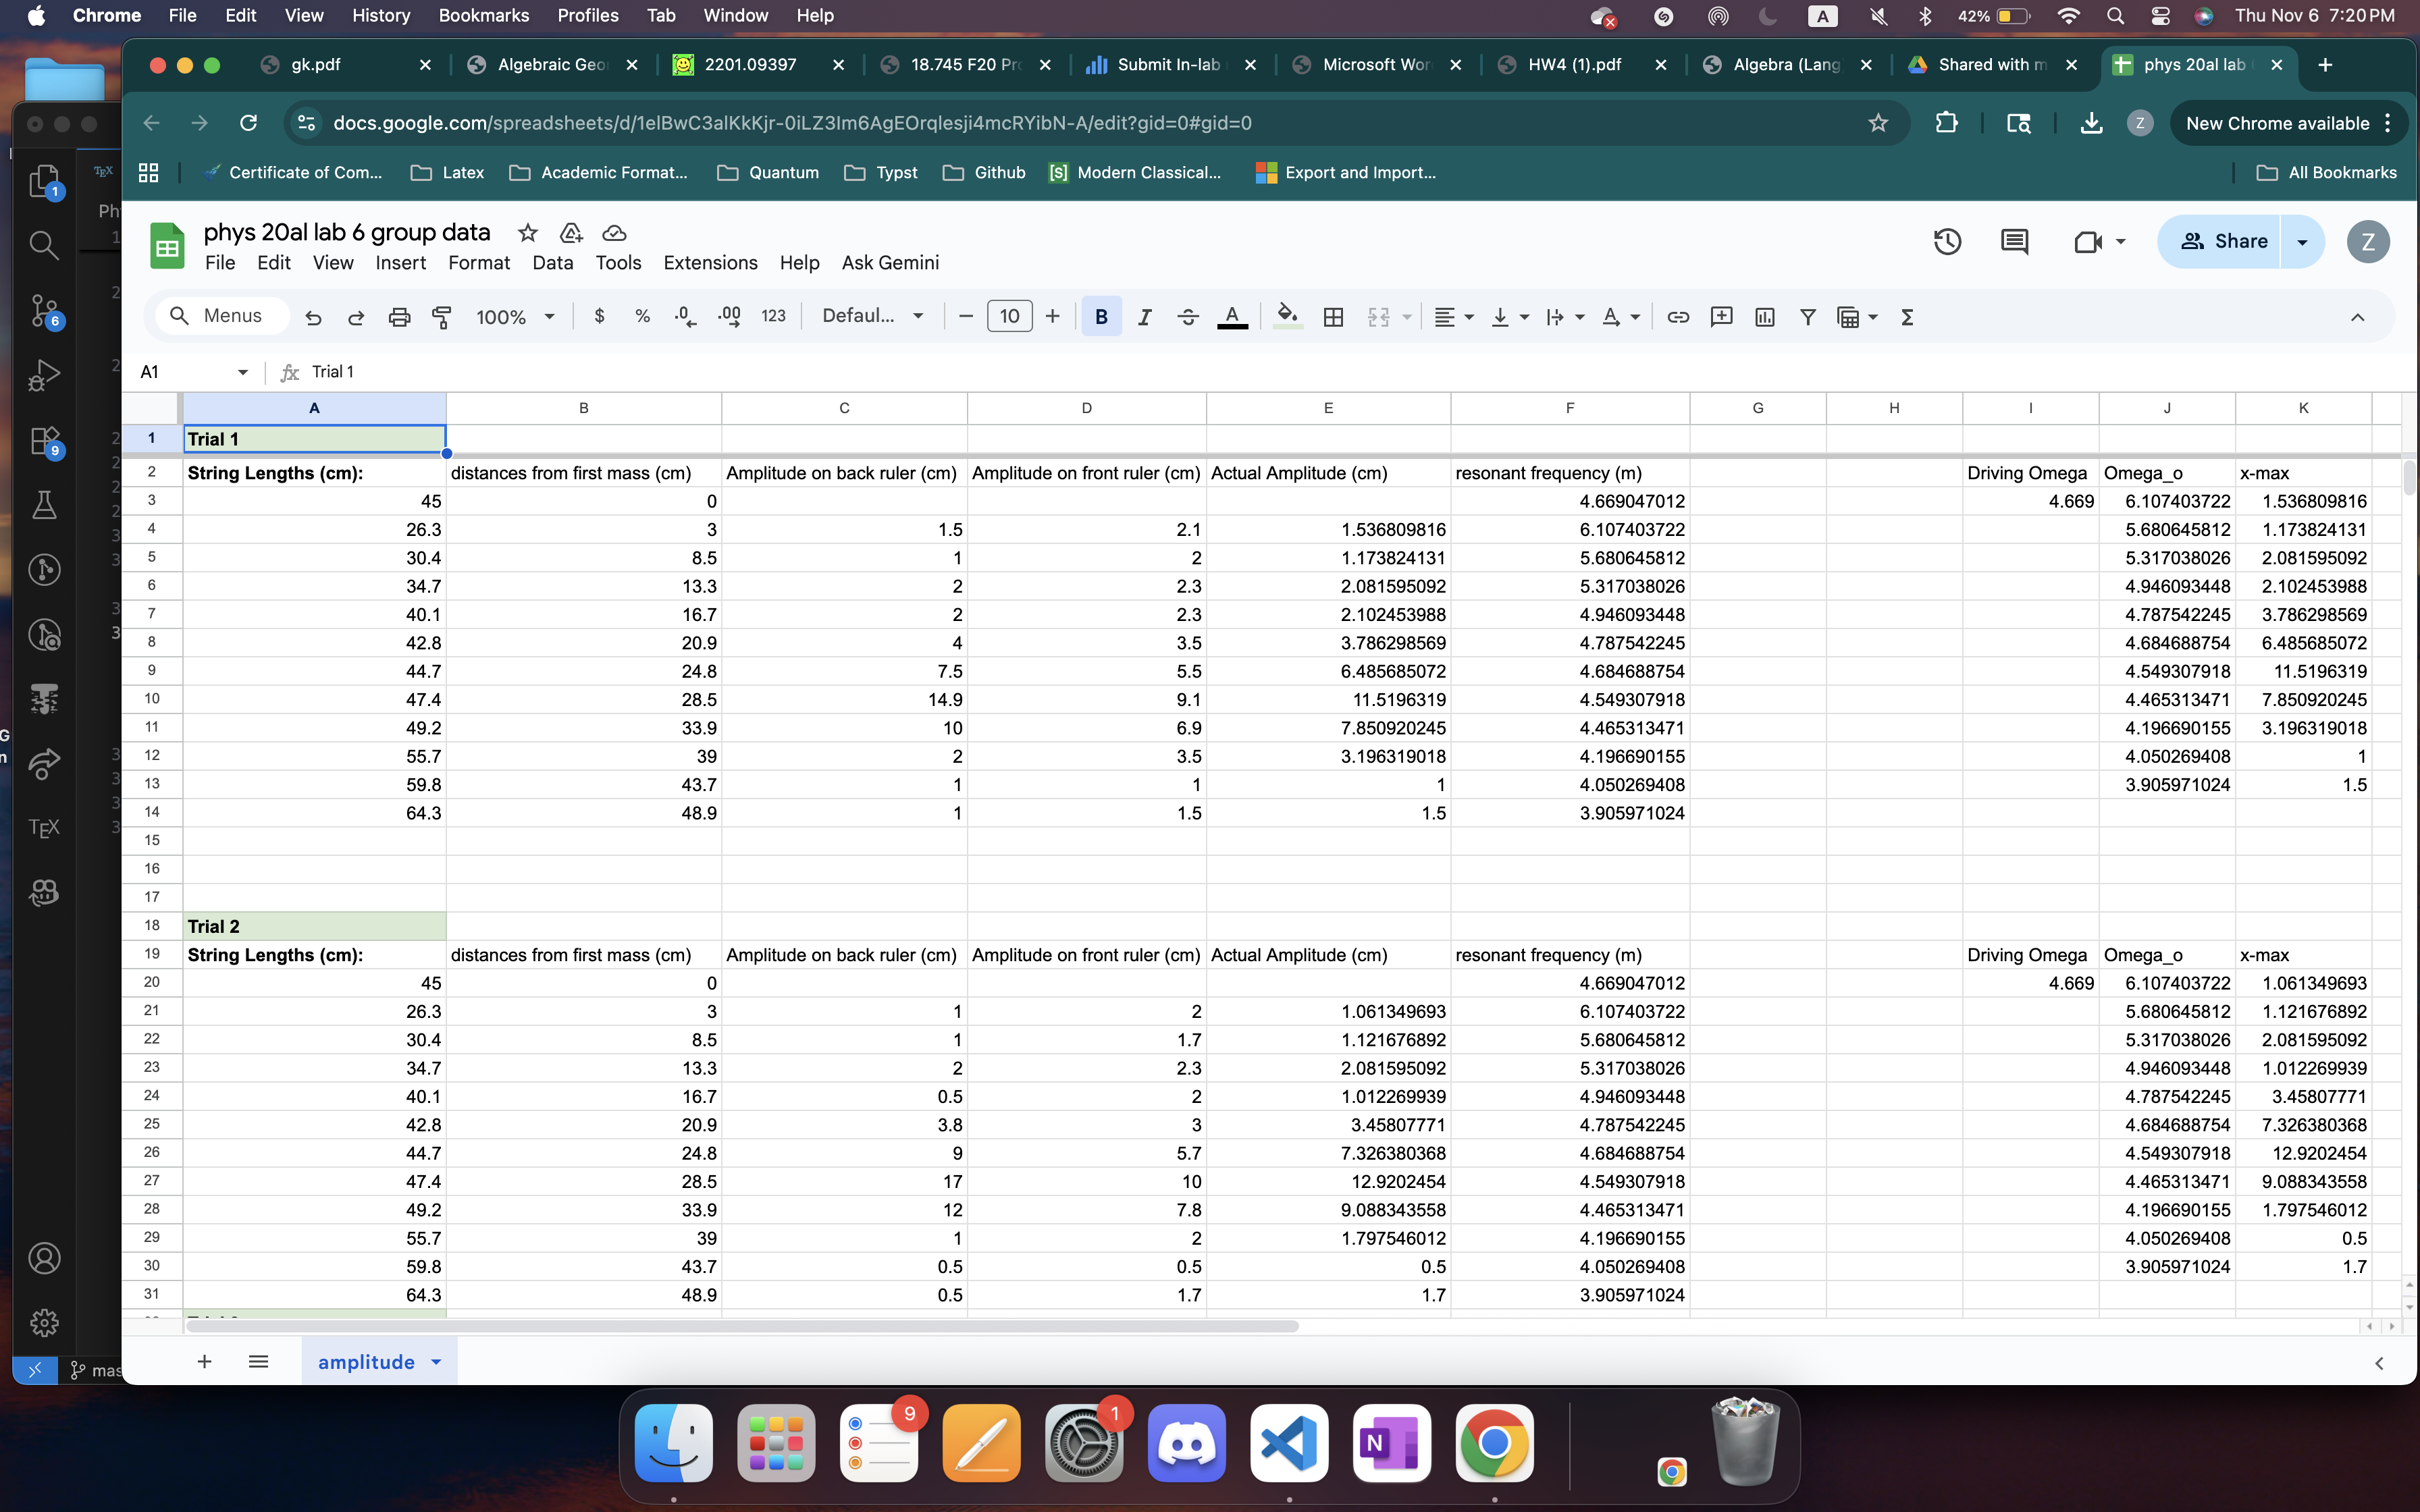
\includegraphics[width=100mm]{amplitude 12.png}
\end{figure}
\begin{figure}[h!]
    \centering
    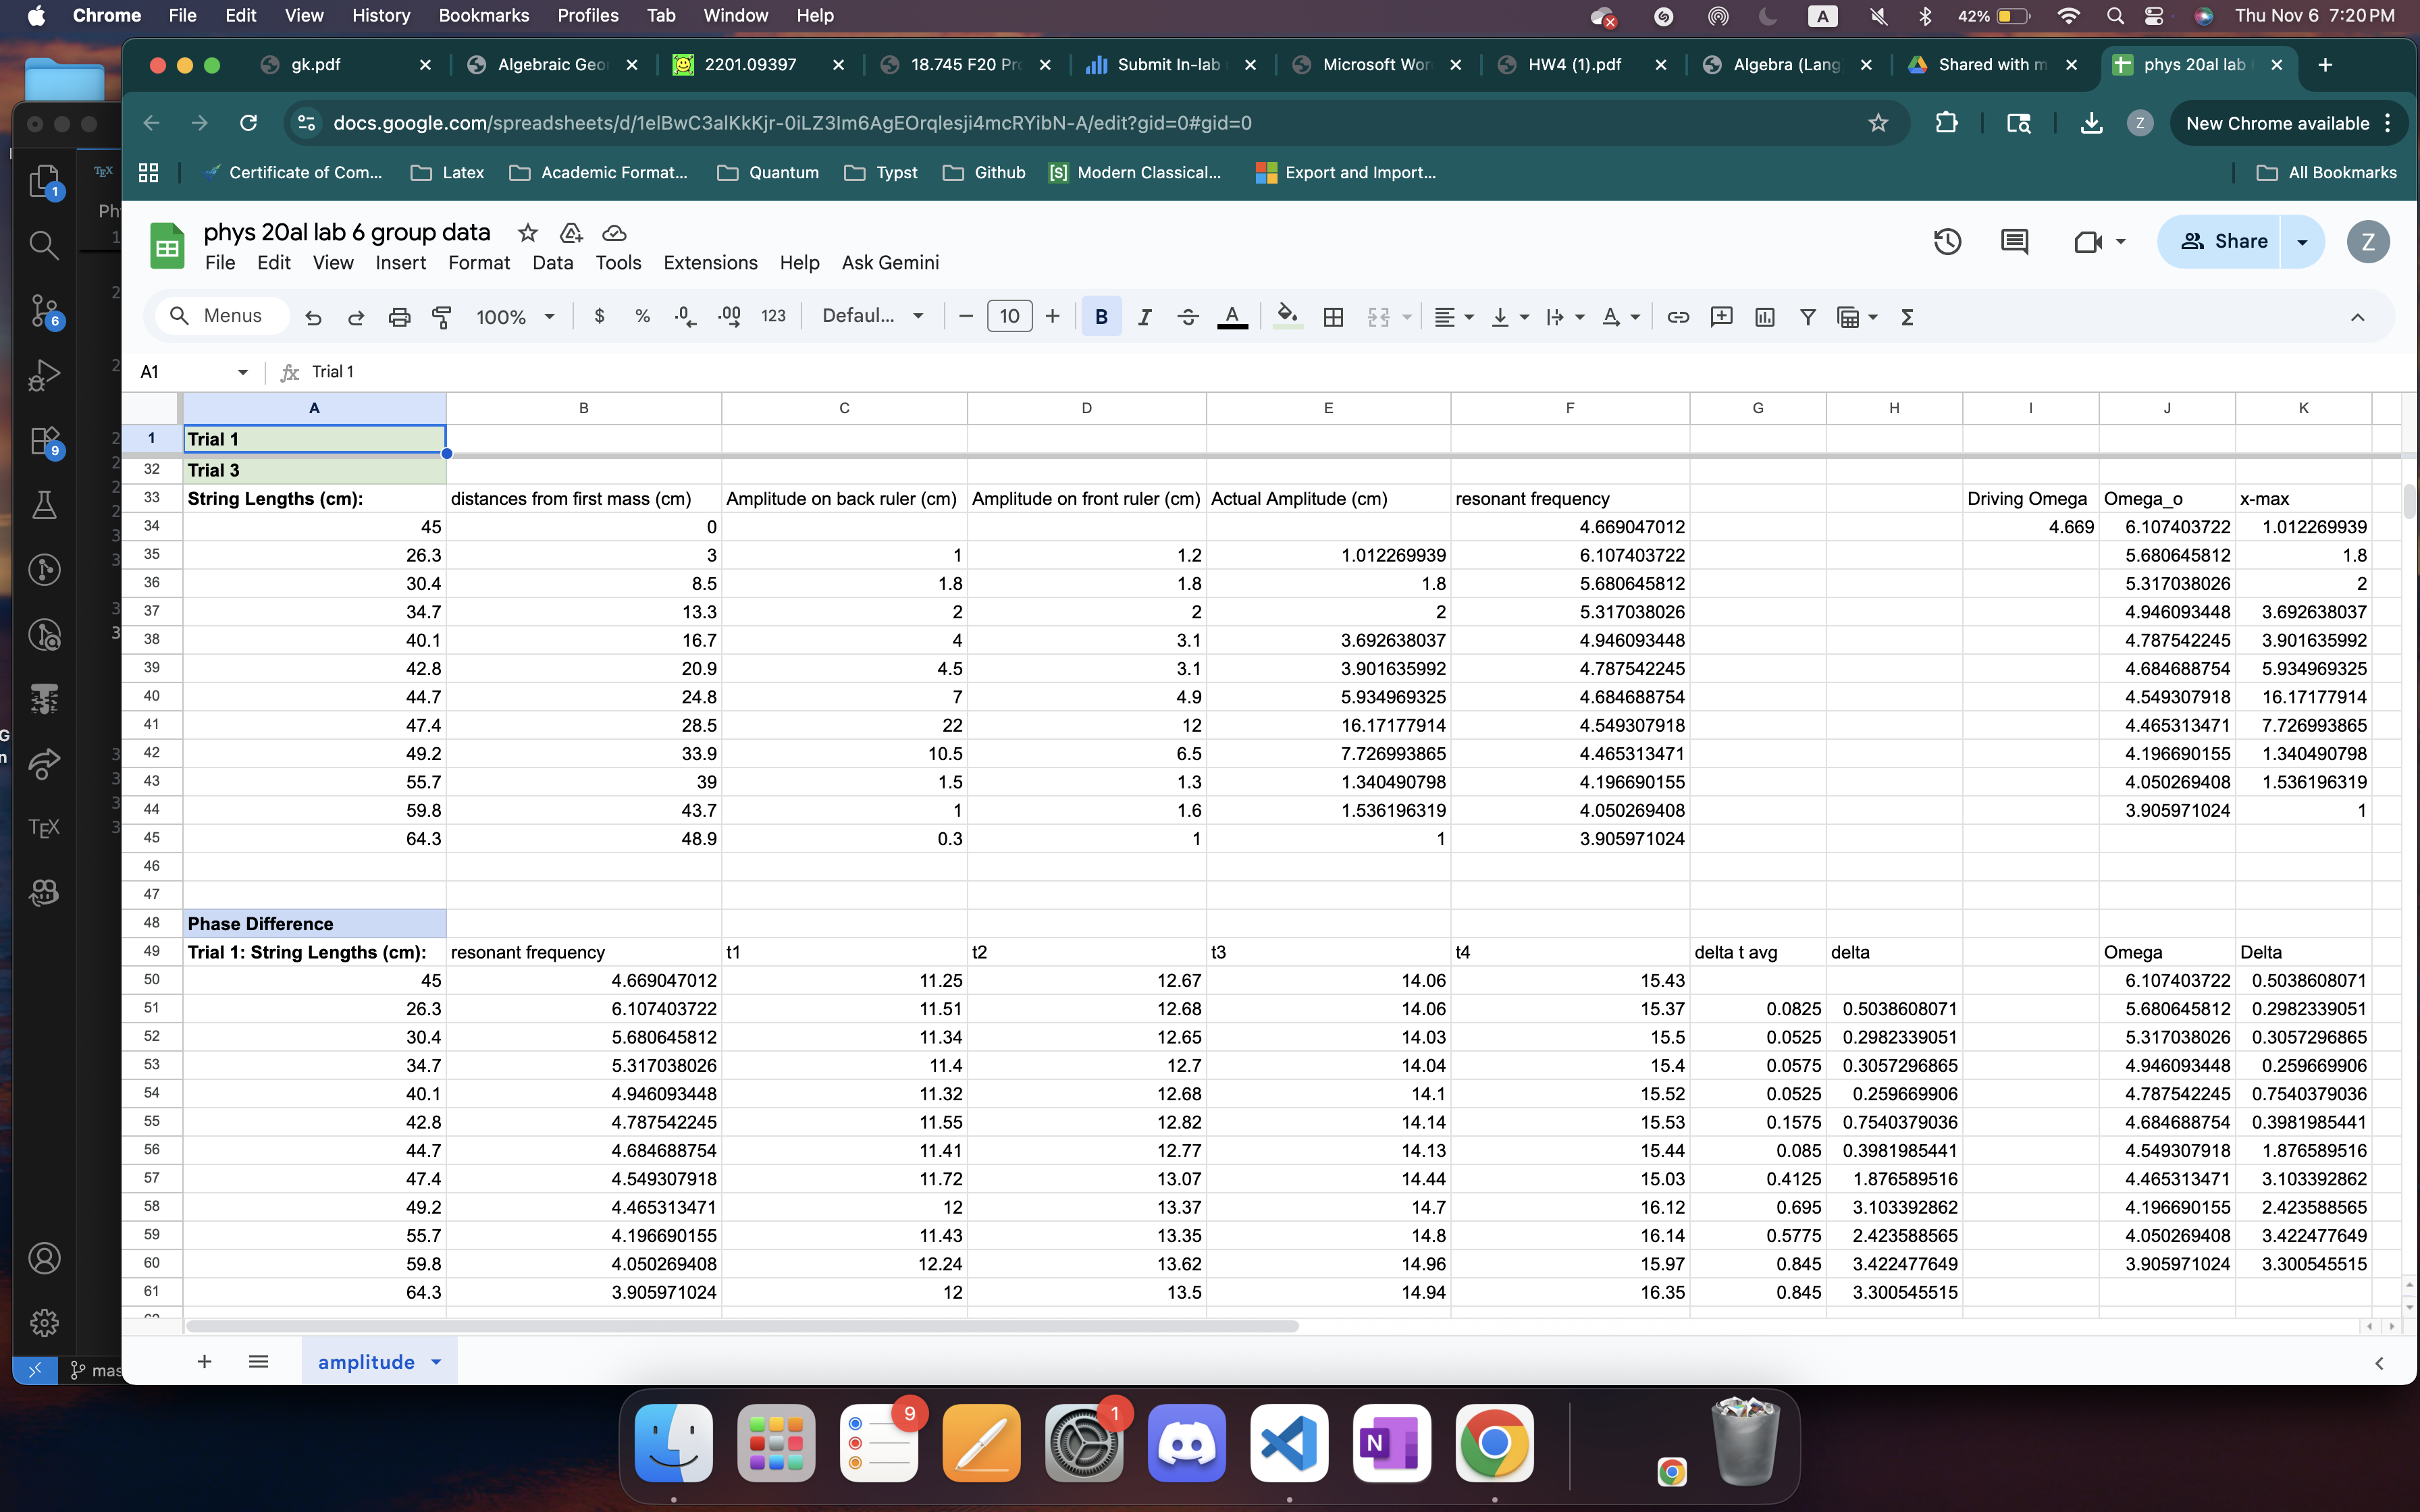
\includegraphics[width=100mm]{amplitude 3 phase 1.png}
\end{figure}
\begin{figure}[h!]
    \centering
    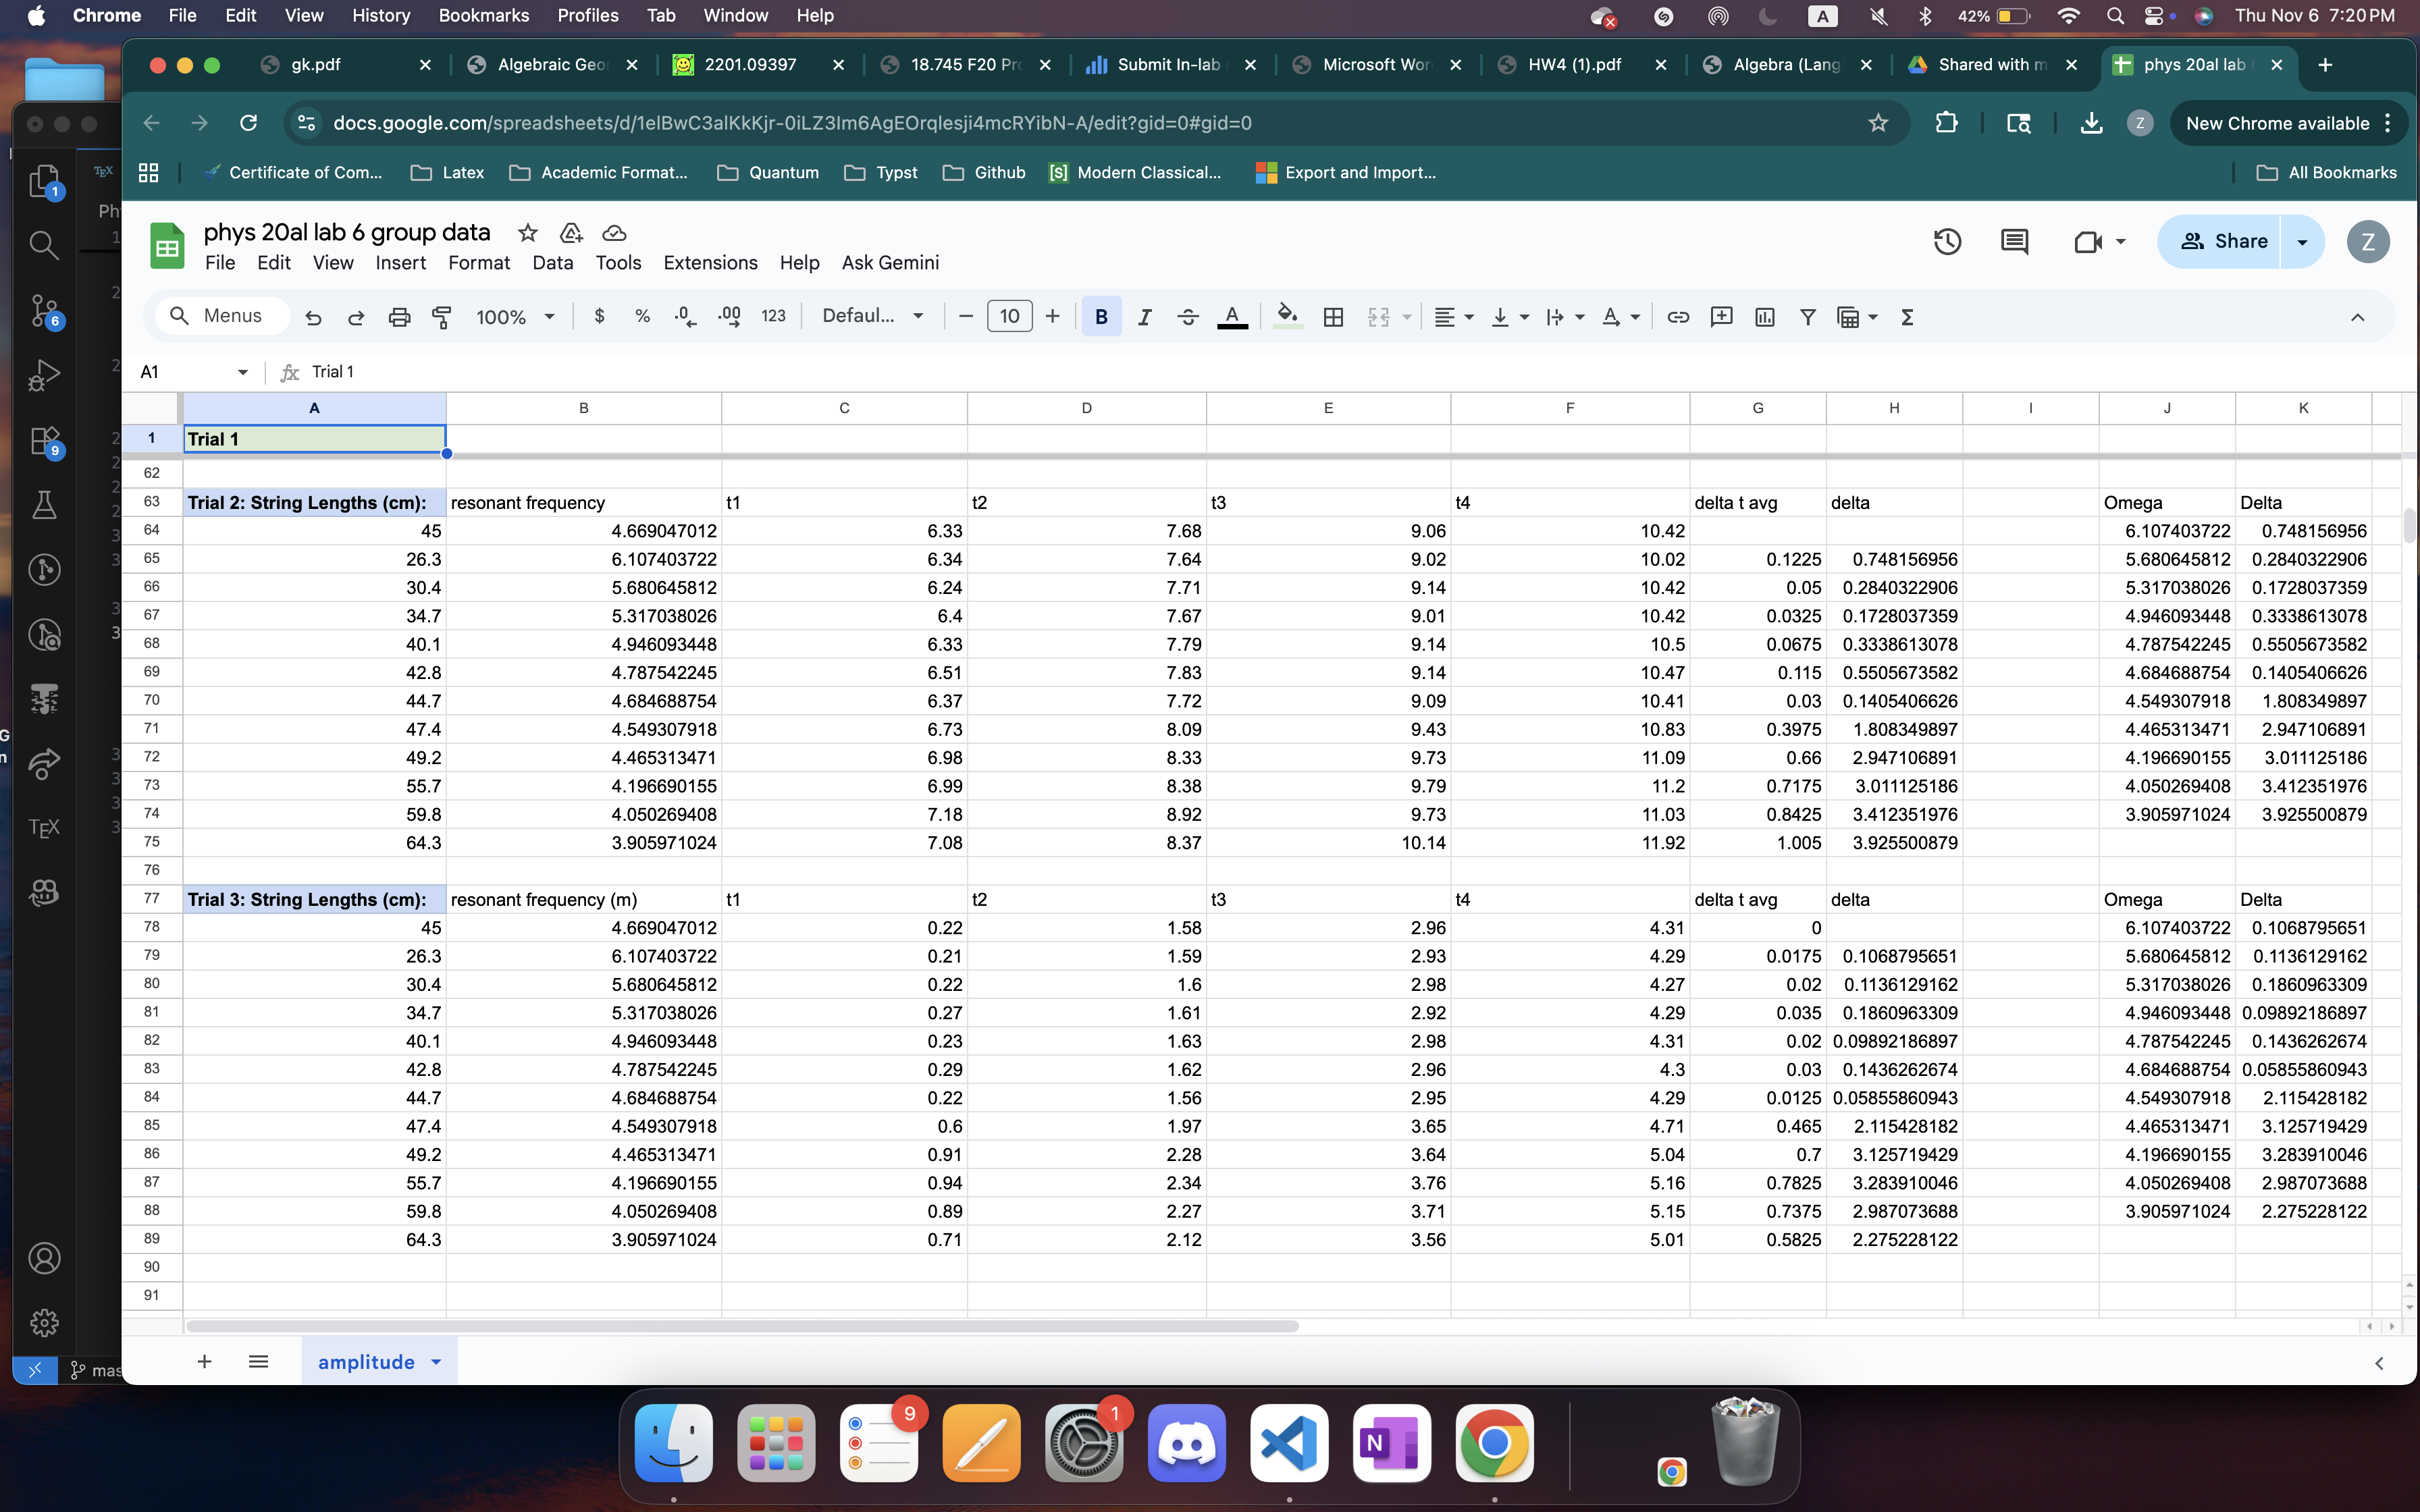
\includegraphics[width=100mm]{phase 23.png}
\end{figure}

\newpage

Here are the tables for amplitude with respect to natural frequencies:
\begin{figure}[h!]
    \centering
    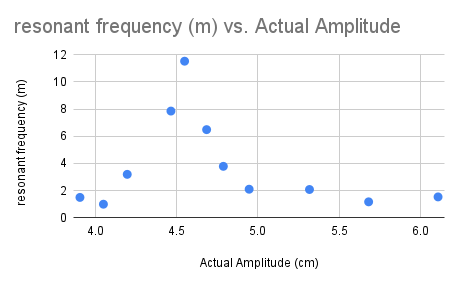
\includegraphics[width=100mm]{resonant frequency (m) vs. Actual Amplitude (cm).png}
\end{figure}
\begin{figure}[h!]
    \centering
    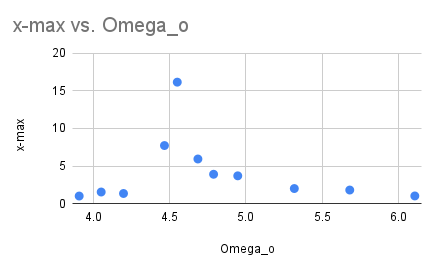
\includegraphics[width=100mm]{x-max vs. Omega_o.png}
\end{figure}
\begin{figure}[h!]
    \centering
    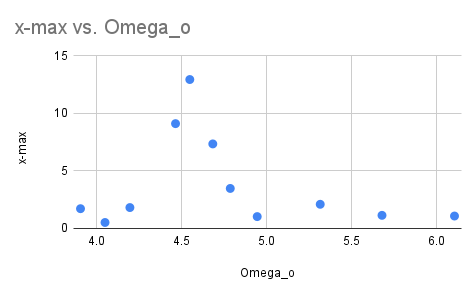
\includegraphics[width=100mm]{x-max vs. Omega_o (1).png}
\end{figure}

\newpage

Here are the tables for phase difference with respect to natural frequencies:
\begin{figure}[h!]
    \centering
    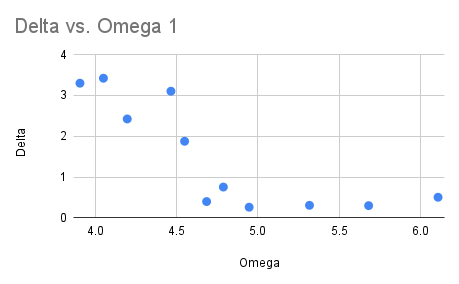
\includegraphics[width=100mm]{Delta vs. Omega 1.png}
\end{figure}
\begin{figure}[h!]
    \centering
    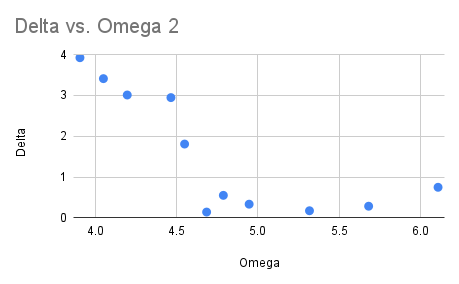
\includegraphics[width=100mm]{Delta vs. Omega 2.png}
\end{figure}
\begin{figure}[h!]
    \centering
    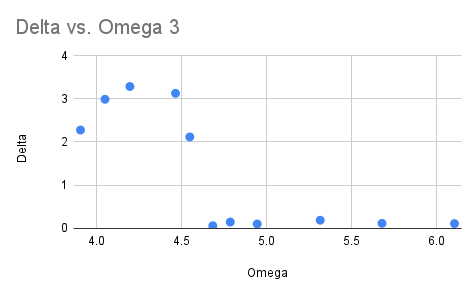
\includegraphics[width=100mm]{Delta vs. Omega 3.png}
\end{figure}

\end{document}